\begin{frame}
  \titlepage
\end{frame}

\begin{frame}{목차}
  \tableofcontents
\end{frame}

\section{문제의식}

\begin{frame}{Chapter 7 소개}
\begin{itemize}
  \item GAT의 핵심 제안은 GCN의 \textbf{정적 정규화 계수} 대신, \textbf{self-attention으로 계산한 가중치}를 쓰는 것이다.
  \item 즉, Transformer에서 널리 알려진 self-attention 아이디어를 \textbf{그래프 이웃 집계}에 반영한 구조라고 볼 수 있다.
  \item 이 self-attention은 BERT, GPT 계열을 성공시킨 Transformer의 핵심 메커니즘이기도 하다.
  \item GAT는 2017년 Veli\v{c}kovi\'{c} et al.이 제안했고, \textbf{기본 설정만으로도 우수한 성능}을 보여 가장 널리 쓰이는 GNN 아키텍처 중 하나가 되었다.
\end{itemize}
\vspace{0.3em}
\begin{block}{이 장의 목표}
graph attention layer가 어떻게 동작하는지 이해하고, NumPy와 PyTorch Geometric으로 직접 구현해 본다.
\end{block}
\end{frame}

\begin{frame}{왜 Attention이 필요한가?}
\begin{itemize}
  \item \textbf{GCN류 모델}: 이웃 노드의 정보를 모아 평균 또는 정규화된 합으로 집계하는 그래프 신경망이다.
  \item \textbf{GAT 모델}: 이웃마다 다른 가중치를 두고, 그 중요도를 attention으로 학습하는 그래프 신경망이다.
  \item GCN류 모델은 이웃을 대체로 균일하게 집계하므로, 중요한 이웃과 덜 중요한 이웃을 구분하기 어렵다.
  \item 그래서 GAT는 노드별/엣지별 중요도를 \textbf{학습된 attention 계수}로 반영한다.
  \item 즉, 이웃 집계에서 ``누구 말을 더 들을지''를 데이터로부터 학습한다.
\end{itemize}
\vspace{0.4em}
\[
\mathbf{h}_i = \left(\sum_{j\in\mathcal{N}(i)} \alpha_{ij}\mathbf{W}\mathbf{h}_j\right)
\]

\begin{block}{수식의 의미}
  \tiny
$\alpha_{ij}$는 노드 $i$가 이웃 $j$의 정보를 얼마나 강하게 반영할지를 나타내는 \textbf{attention score}다.
즉, 각 이웃의 메시지 $\mathbf{W}\mathbf{h}_j$에 서로 다른 가중치를 곱해 합치므로, 중요한 이웃일수록 최종 표현 $\mathbf{h}_i$에 더 크게 기여한다.
\end{block}
\end{frame}

\begin{frame}{핵심 아이디어}
\begin{block}{GAT의 관점}
메시지 패싱은 같지만, 이웃마다 가중치 $\alpha_{ij}$를 다르게 주어 더 유의미한 구조를 강조한다.
\end{block}
\vspace{0.4em}
\begin{itemize}
  \item \textbf{장점}: 중요 이웃 선택, 해석성 향상(계수 확인 가능)
  \item \textbf{비용}: 파라미터/연산 증가, 데이터셋 성질에 따라 불안정 가능
\end{itemize}
\end{frame}

\begin{frame}{실습 노트북 소개}
\begin{itemize}
  \item \texttt{chapter7\_annotated.ipynb}는 실습 코드에 교재 설명을 삽입한 통합 버전이다.
  \item 목표는 ``코드를 실행하는 것''보다 ``각 셀이 왜 필요한지 이해하는 것''
  \item 슬라이드 파일과 함께 제공
\end{itemize}
\vspace{0.4em}
\begin{block}{학습 포인트}
attention 계수 생성, toy example 수식-코드 매칭, 데이터셋별 성능 차이, degree 기반 한계 해석
\end{block}
\end{frame}

\begin{frame}{이 장에서 다룰 내용}
\begin{enumerate}
  \item graph attention layer 소개
  \item NumPy로 graph attention layer 구현
  \item PyTorch Geometric으로 GAT 구현
\end{enumerate}
\vspace{0.3em}
\begin{itemize}
  \item 후반부에서는 Cora와 CiteSeer에서 결과를 분석하고, GCN과의 차이도 함께 해석한다.
  \item 마지막 목표는 scratch 구현, PyG 구현, 그리고 graph data용 error analysis 관점까지 익히는 것이다.
\end{itemize}
\end{frame}

\begin{frame}{먼저 구분: GAN vs GAT}
\begin{itemize}
  \item \textbf{GAN}: 생성자와 판별자가 경쟁하는 생성 모델
  \item \textbf{GAT}: 그래프 이웃의 중요도를 attention으로 학습하는 분류/표현학습 모델
  \item 이 장의 핵심 질문은 ``무엇을 생성할까''가 아니라 ``어떤 이웃을 더 크게 반영할까''이다.
\end{itemize}
\end{frame}

\section{GAT 동작 원리}

\begin{frame}{Attention score 계산 절차}
\begin{enumerate}
  \item Linear transformation
  \item Activation function
  \item Softmax normalization
  \item Multi-head attention
  \item Improved graph attention layer
\end{enumerate}
\vspace{0.3em}
\begin{block}{핵심 메시지}
GAT에서는 attention score를 외부 규칙으로 정하지 않고, 입력된 노드 표현들끼리 서로 비교하여 직접 계산한다.
즉, 노드 $i$와 이웃 $j$의 특징으로부터 $\alpha_{ij}$를 만들기 때문에, 입력 자체가 스스로 중요도를 결정한다는 뜻에서 self-attention이라고 부른다.
\end{block}
\end{frame}

\begin{frame}{1. Linear transformation}
\small
첫 단계는 중심 노드 $i$와 이웃 노드 $j$의 특징을 같은 가중치 행렬로 변환한 뒤, 이를 이어 붙여 attention 계산의 입력으로 만드는 것이다.
\[
a_{ij} = \mathbf{W}_{att}^{\top}[\mathbf{W}\mathbf{x}_i \, \| \, \mathbf{W}\mathbf{x}_j]
\]
\vspace{0.3em}
\begin{itemize}
  \item $i$: 중심 노드, $j$: 이웃 노드
  \item $\mathbf{x}_i, \mathbf{x}_j$: 두 노드의 원래 입력 특징 벡터
  \item $\mathbf{W}$: 모든 노드에 공통으로 적용되는 shared weight matrix
  \item $\mathbf{W}\mathbf{x}_i, \mathbf{W}\mathbf{x}_j$: 선형변환 뒤 얻는 hidden vector
  \item $[\mathbf{W}\mathbf{x}_i \| \mathbf{W}\mathbf{x}_j]$: 두 hidden vector를 이어 붙인 벡터
  \item $\mathbf{W}_{att}$: 이어 붙인 벡터를 attention score로 바꾸는 추가 학습 가중치
  \item $a_{ij}$: activation function에 넣기 전의 선형 attention score
\end{itemize}
\end{frame}

\begin{frame}{2. Activation function}
\small
앞 단계의 선형 score $a_{ij}$를 activation function에 통과시켜 raw attention score를 만든다.
\[
e_{ij} = \text{LeakyReLU}(a_{ij})
\]
\vspace{0.3em}
\begin{itemize}
  \item $a_{ij}$: 선형변환만 거친 상태의 점수
  \item $e_{ij}$: LeakyReLU를 통과한 뒤의 raw attention score
  \item activation을 넣는 이유는 점수 계산에 비선형성을 주어 더 유연한 중요도 비교가 가능하게 하기 위해서다.
  \item ReLU와 달리 음수 구간도 작은 기울기를 남겨, 중요도가 낮은 이웃이라도 학습 신호가 완전히 끊기지 않는다.
  \item 직관적으로는 ``노드 $i$가 이웃 $j$를 얼마나 주목해야 하는가''를 더 표현력 있게 점수화하는 단계다.
\end{itemize}
\end{frame}

\begin{frame}{왜 LeakyReLU를 쓰는가?}
\small
\begin{columns}[T,totalwidth=\textwidth]
\begin{column}{0.56\textwidth}
\begin{itemize}
  \item ReLU는 음수 입력을 모두 0으로 보내므로, attention score가 음수인 구간에서는 정보와 기울기가 너무 쉽게 사라질 수 있다.
  \item LeakyReLU는 음수 구간에 작은 기울기($\alpha x$)를 남겨 score의 순서와 차이를 조금 더 유지한다.
  \item 그래서 초기 학습 단계에서 특정 이웃이 덜 중요해 보여도, 나중에 다시 중요해질 가능성을 열어 둔다.
\end{itemize}
\vspace{0.3em}
\[
\text{LeakyReLU}(x)=
\begin{cases}
x, & x \ge 0 \\
\alpha x, & x < 0
\end{cases}
\]
\end{column}
\begin{column}{0.44\textwidth}
\centering
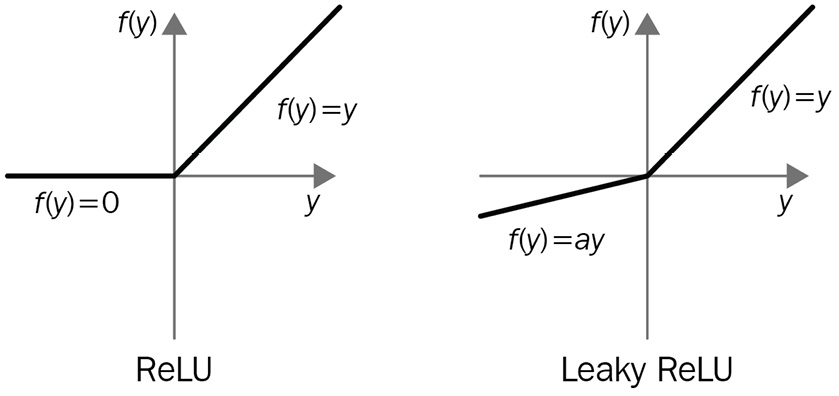
\includegraphics[width=\textwidth,height=0.56\textheight,keepaspectratio]{images/B19153_07_001.jpg}
\vspace{0.3em}

\small ReLU vs LeakyReLU (교재 그림 7.1): 음수 구간에서의 차이를 시각적으로 보여준다.
\end{column}
\end{columns}
\end{frame}

\begin{frame}{3. Softmax normalization}
\small
같은 중심 노드 $i$의 이웃들 사이에서 softmax를 적용해 attention score를 확률처럼 정규화한다.
\[
\alpha_{ij} = softmax_j(e_{ij}) = \frac{\exp(e_{ij})}{\sum_{k\in\mathcal{N}(i)}\exp(e_{ik})}
\]
\vspace{0.3em}
\begin{itemize}
  \item $\mathcal{N}(i)$: 노드 $i$에 연결된 이웃들의 집합
  \item $k$: 노드 $i$의 이웃들을 하나씩 가리키는 인덱스
  \item $\alpha_{ij}$: 정규화된 attention coefficient로, 노드 $i$가 이웃 $j$의 정보를 얼마나 반영할지 뜻한다.
  \item softmax를 쓰면 노드 $i$의 모든 이웃에 대한 계수 합이 1이 되어 상대적 중요도를 비교할 수 있다.
  \item 즉, ``누가 더 중요한 이웃인가''를 ranking 가능한 비율로 바꿔 주는 단계다.
  \item toy example의 \texttt{softmax2D(E, 1)}가 바로 이 단계다.
\end{itemize}
\end{frame}

\begin{frame}{4. Multi-head attention}
\small
Vaswani et al. (2017)이 Transformer에서 사용한 것처럼, attention을 한 번만 계산하지 않고 여러 head에서 병렬로 계산해 표현력을 높인다.
\vspace{0.3em}
\begin{itemize}
  \item $m$: 여러 attention head 중 하나를 가리키는 인덱스
  \item $\mathbf{W}^{(m)}$, $\alpha_{ij}^{(m)}$: $m$번째 head가 따로 학습한 변환 행렬과 attention coefficient
  \item 각 head는 하나의 embedding $\mathbf{h}_i^{(m)}$를 만든다.
  \item 각 head는 같은 이웃을 보더라도 조금 다른 기준으로 중요도를 계산할 수 있다.
  \item 여러 head의 결과를 합치는 방법은 두 가지다.
  \item \textbf{Averaging}: 마지막 레이어에서 주로 사용하며, 여러 head 출력을 평균낸다.
  \item \textbf{Concatenation}: hidden layer에서 주로 사용하며, 여러 head 출력을 이어 붙인다.
\end{itemize}
\end{frame}

\begin{frame}{Multi-head 결합 방식}
\small
\begin{columns}[T,totalwidth=\textwidth]
\begin{column}{0.52\textwidth}
\begin{block}{Averaging}
\[
\mathbf{h}_i = \frac{1}{n}\sum_{k=1}^{n}\mathbf{h}_i^{k}
= \frac{1}{n}\sum_{k=1}^{n}\sum_{j\in\mathcal{N}_i}\alpha_{ij}^{k}\mathbf{W}^{k}\mathbf{x}_j
\]
\end{block}
\vspace{0.2em}
\begin{block}{Concatenation}
\[
\mathbf{h}_i =
\mathop{\Vert}_{k=1}^{n}\mathbf{h}_i^{k}
= \mathop{\Vert}_{k=1}^{n}\sum_{j\in\mathcal{N}_i}\alpha_{ij}^{k}\mathbf{W}^{k}\mathbf{x}_j
\]
\end{block}
\vspace{0.2em}
\begin{itemize}
  \item hidden layer: 보통 concatenation
  \item 마지막 layer: 보통 averaging
\end{itemize}
\end{column}
\begin{column}{0.48\textwidth}
\centering
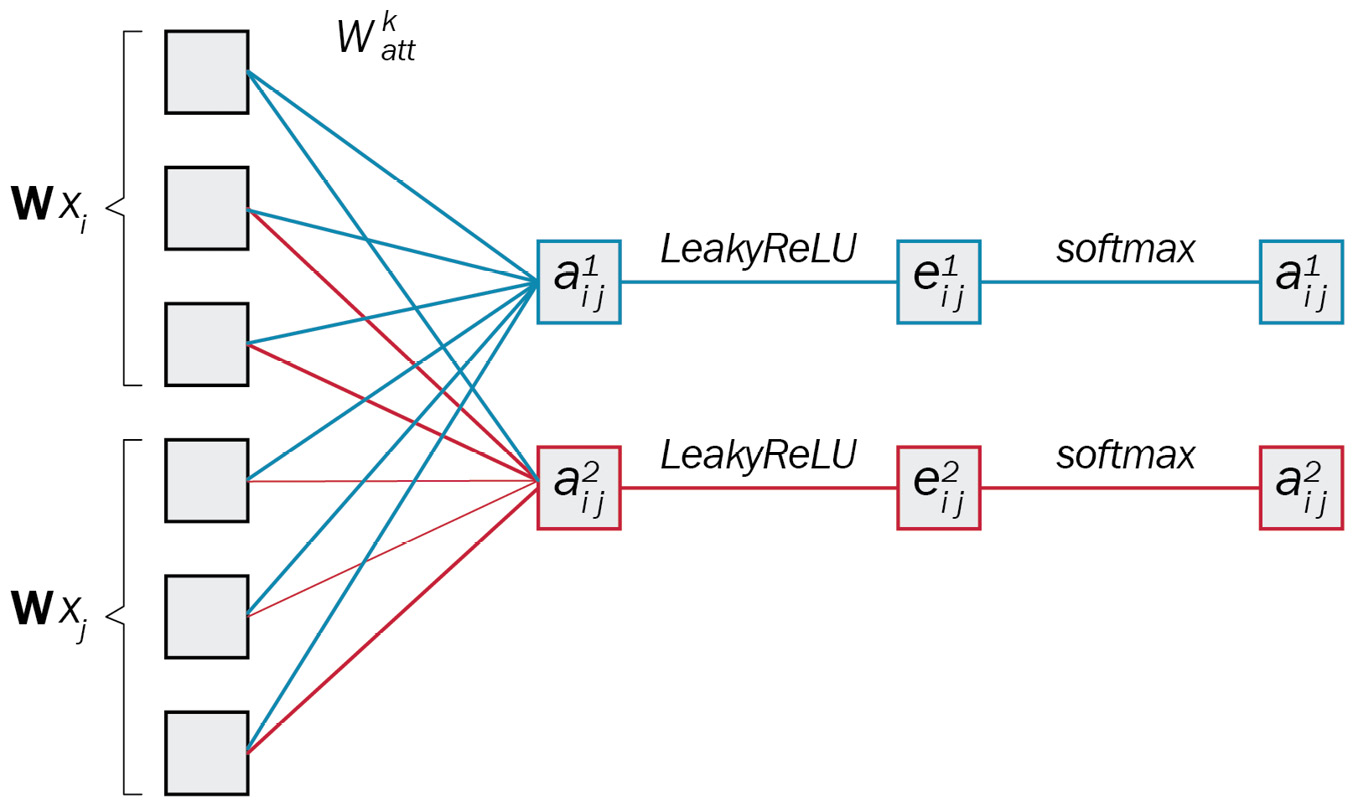
\includegraphics[width=\textwidth,height=0.62\textheight,keepaspectratio]{images/B19153_07_002.jpg}
\vspace{0.3em}

\small 교재 그림 7.2: 여러 attention head의 결과를 결합하는 흐름
\end{column}
\end{columns}
\end{frame}

\begin{frame}{5. Improved graph attention layer}
\small
Brody et al. (2021)은 원래 GAT가 \textbf{static attention}만 계산한다고 지적했다.
\vspace{0.3em}
\begin{itemize}
  \item attention의 상대적 순위가 입력 쌍에 따라 충분히 유연하게 바뀌지 못하는 경우가 있다는 것이다.
  \item 이로 인해 단순한 그래프 문제도 원래 GAT로는 표현하지 못하는 사례가 생길 수 있다.
  \item 이를 개선하기 위해 제안된 것이 \textbf{GATv2}이며, Brody et al.은 이를 \textbf{dynamic attention}이라고 설명한다.
  \item 실습에서 \texttt{GATv2Conv}를 쓰는 이유도 바로 이 더 높은 표현력 때문이다.
\end{itemize}
\end{frame}

\begin{frame}{GAT와 GATv2의 차이}
\small
\begin{block}{Original GAT}
\[
\alpha_{ij} =
\frac{
\exp\left(
\text{LeakyReLU}\left(
\mathbf{W}_{att}^{\top}
[\mathbf{W}\mathbf{x}_i \| \mathbf{W}\mathbf{x}_j]
\right)
\right)
}{
\sum_{k\in\mathcal{N}_i}
\exp\left(
\text{LeakyReLU}\left(
\mathbf{W}_{att}^{\top}
[\mathbf{W}\mathbf{x}_i \| \mathbf{W}\mathbf{x}_k]
\right)
\right)
}
\]
\end{block}
\vspace{0.3em}
\begin{block}{GATv2}
\[
\alpha_{ij} =
\frac{
\exp\left(
\mathbf{W}_{att}^{\top}
\text{LeakyReLU}\left(
\mathbf{W}[\mathbf{x}_i \| \mathbf{x}_j]
\right)
\right)
}{
\sum_{k\in\mathcal{N}_i}
\exp\left(
\mathbf{W}_{att}^{\top}
\text{LeakyReLU}\left(
\mathbf{W}[\mathbf{x}_i \| \mathbf{x}_k]
\right)
\right)
}
\]
\end{block}
\vspace{0.3em}
\begin{itemize}
  \item 핵심 차이는 \textbf{선형변환과 attention projection의 순서}다.
  \item \textbf{GAT}: 각 노드를 먼저 따로 변환한 뒤 score를 만든다.
  \item \textbf{GATv2}: concat한 입력 전체에 변환을 적용한 뒤 score를 만든다.
  \item 그래서 GATv2는 입력 쌍 $(i,j)$에 따라 attention 순위가 더 유연하게 바뀔 수 있다.
  \item 결론: 실전에서는 보통 \textbf{GATv2를 우선 선택}하는 편이 낫다.
\end{itemize}
\end{frame}

\begin{frame}{이제부터는 실습 노트북으로 본다}
\begin{itemize}
  \item 지금까지는 graph attention layer의 원리를 교재 기준으로 정리했다.
  \item 이제부터는 \texttt{chapter7\_annotated.ipynb}의 \textbf{핵심 실습 흐름}을 따라가며, 이 이론이 코드에서 어떻게 구현되는지 본다.
  \item 순서는 toy example으로 attention 계산을 확인하고, 그 다음 PyTorch Geometric의 \texttt{GATv2Conv} 구현과 실험 결과를 해석하는 방식이다.
\end{itemize}
\vspace{0.3em}
\begin{block}{전환 포인트}
이제부터 슬라이드는 ``교재 설명''보다 ``ipynb의 핵심 셀 흐름''에 맞춰 읽으면 된다.
\end{block}
\end{frame}

\begin{frame}{ipynb 도입부: 목적과 용어 정리}
\begin{itemize}
  \item 노트북은 \textbf{교재 설명 + 실행 가능한 실습 코드}를 한 흐름으로 묶어 둔 통합 버전이다.
  \item 먼저 이 노트북에서 볼 것은 attention coefficient가 어떻게 만들어지는지, 그리고 toy example의 수식과 코드가 어떻게 대응되는지다.
  \item 도입부에서는 용어 혼동을 막기 위해 \textbf{GAN이 아니라 GAT}라는 점도 먼저 정리한다.
\end{itemize}
\vspace{0.3em}
\begin{block}{이후 흐름}
환경 설정과 간단한 입력 준비를 거친 뒤, 바로 4노드 toy example로 들어가 attention 계산을 손으로 추적한다.
\end{block}
\end{frame}

\begin{frame}[fragile]{노트북 1부: 4노드 toy 예제}
\begin{itemize}
  \item 노트북은 방금 본 1--3단계를 작은 adjacency matrix에서 직접 구현한다.
  \item \texttt{A, X, W, W\_att}를 만든 뒤, 연결된 쌍의 점수 $e_{ij}$를 구하고 정규화한다.
\end{itemize}
\vspace{0.3em}
\begin{lstlisting}
connections = np.where(A > 0)
a = W_att @ np.concatenate([
    (X @ W.T)[connections[0]],
    (X @ W.T)[connections[1]]
], axis=1).T

e = leaky_relu(a)
E = np.zeros(A.shape)
E[connections[0], connections[1]] = e[0]
W_alpha = softmax2D(E, 1)
\end{lstlisting}
\end{frame}

\begin{frame}{toy example를 읽는 순서}
\begin{enumerate}
  \item $A, X, W, W_{att}$로 입력과 파라미터를 준비한다.
  \item Linear transformation으로 $\mathbf{W}\mathbf{h}_i$를 만든다.
  \item Activation function과 softmax로 $e_{ij}\rightarrow\alpha_{ij}$를 만든다.
  \item attention 가중합으로 최종 표현 $H$를 얻는다.
\end{enumerate}
\vspace{0.3em}
\begin{block}{발표 포인트}
이 예제를 이해하면 \texttt{GATv2Conv}의 내부 동작이 블랙박스처럼 보이지 않는다.
\end{block}
\end{frame}

\begin{frame}{교재 그림: Attention 계산 직관 (1)}
\centering
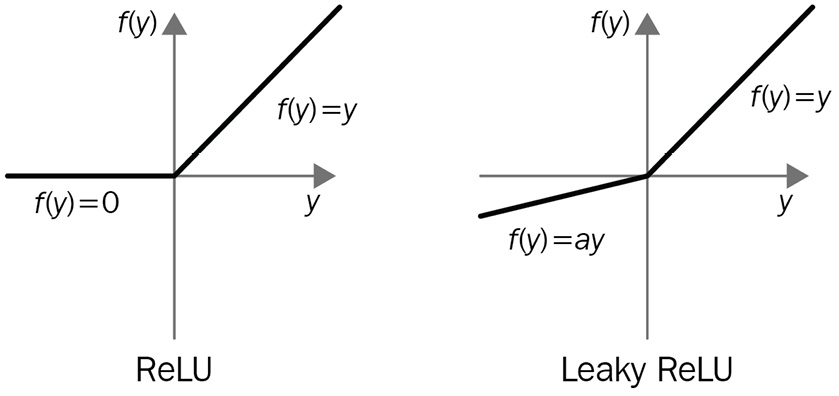
\includegraphics[width=\textwidth,height=0.72\textheight,keepaspectratio]{images/B19153_07_001.jpg}
\vspace{0.2em}

\small Figure 7.1 (교재): 이웃별 중요도 부여 개념
\end{frame}

\begin{frame}{교재 그림: Attention 계산 직관 (2)}
\centering
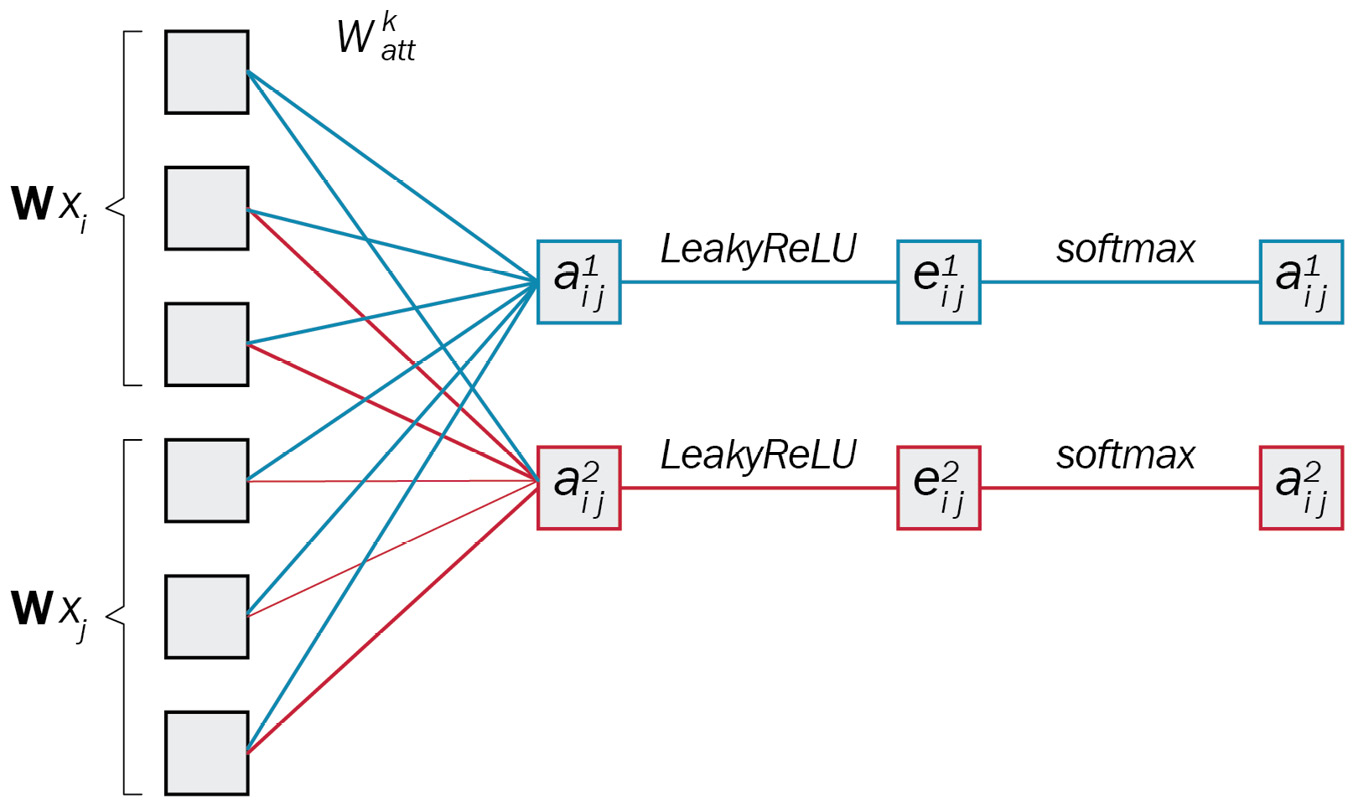
\includegraphics[width=\textwidth,height=0.72\textheight,keepaspectratio]{images/B19153_07_002.jpg}
\vspace{0.2em}

\small Figure 7.2 (교재): 계수 정규화와 메시지 집계
\end{frame}

\section{PyG 실습}

\begin{frame}[fragile]{GATv2 모델 구현 (PyTorch Geometric)}
\small
\begin{lstlisting}
class GAT(torch.nn.Module):
    def __init__(self, dim_in, dim_h, dim_out, heads=8):
        super().__init__()
        self.gat1 = GATv2Conv(dim_in, dim_h, heads=heads)
        self.gat2 = GATv2Conv(dim_h*heads, dim_out, heads=1)

    def forward(self, x, edge_index):
        h = F.dropout(x, p=0.6, training=self.training)
        h = self.gat1(h, edge_index)
        h = F.elu(h)
        h = F.dropout(h, p=0.6, training=self.training)
        h = self.gat2(h, edge_index)
        return F.log_softmax(h, dim=1)
\end{lstlisting}
\end{frame}

\begin{frame}{PyG 구현에서 볼 핵심 3개}
\begin{itemize}
  \item \textbf{Multi-head}: 서로 다른 관점으로 이웃 중요도를 보게 해 표현력을 높인다.
  \item \textbf{Dropout 두 번}: 입력 특징과 은닉 표현 모두 regularization해 과적합을 줄인다.
  \item \textbf{Train mask 학습}: 손실은 라벨이 있는 훈련 노드에 대해서만 계산된다.
\end{itemize}
\vspace{0.3em}
\[
\mathcal{L} = -\sum_{i\in \mathcal{V}_{train}} \log p(y_i \mid x_i, G)
\]
\end{frame}

\begin{frame}{실험 설정 요약}
\begin{itemize}
  \item 데이터셋: Cora, CiteSeer (Planetoid)
  \item 옵티마이저: Adam ($\text{lr}=0.01$, weight decay $=0.01$)
  \item 학습 epoch: 100
  \item 드롭아웃: 0.6
  \item 다중 헤드: 첫 층 8 heads, 출력층 1 head
\end{itemize}
\end{frame}

\begin{frame}{교재 그림: GAT/GATv2 레이어 구조 (1)}
\centering
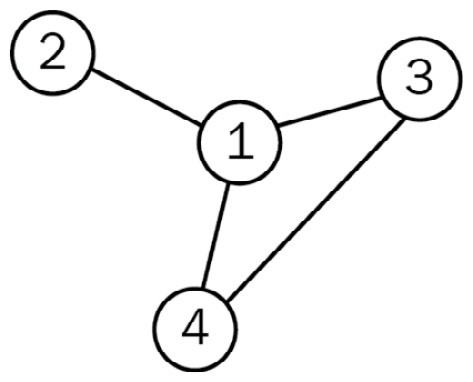
\includegraphics[width=\textwidth,height=0.72\textheight,keepaspectratio]{images/B19153_07_003.jpg}
\vspace{0.2em}

\small Figure 7.3 (교재): GAT 레이어의 정보 흐름
\end{frame}

\begin{frame}{교재 그림: GAT/GATv2 레이어 구조 (2)}
\centering
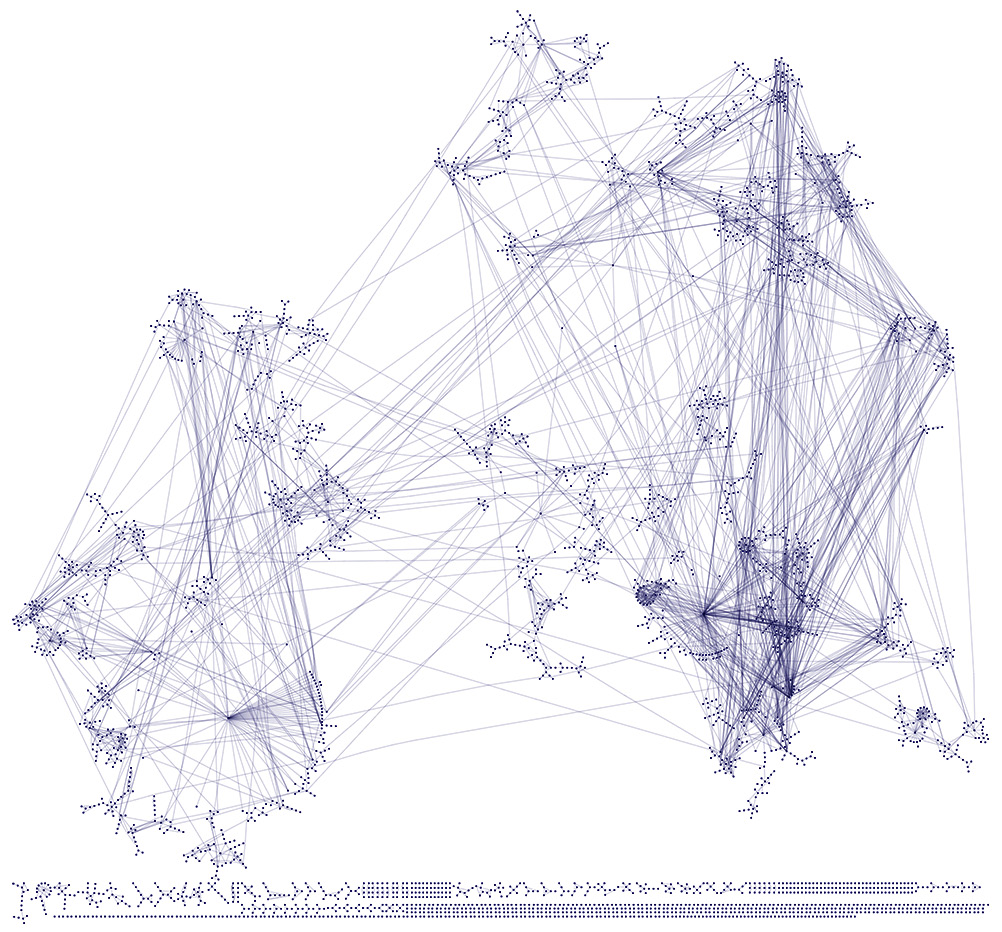
\includegraphics[width=\textwidth,height=0.72\textheight,keepaspectratio]{images/B19153_07_004.jpg}
\vspace{0.2em}

\small Figure 7.4 (교재): multi-head attention 구성
\end{frame}

\begin{frame}{주요 결과 (노트북 실행값)}
\begin{itemize}
  \item Cora: \textbf{GAT test accuracy = 81.10\%}
  \item CiteSeer: \textbf{GAT test accuracy = 68.10\%}
\end{itemize}
\vspace{0.4em}
\begin{block}{해석 포인트}
데이터셋별 구조/특징 분포가 달라 attention이 주는 이득과 일반화 성능이 다르게 나타난다.
\end{block}
\end{frame}

\begin{frame}{결과를 읽는 법}
\begin{itemize}
  \item 정확도 차이는 모델 구조뿐 아니라 그래프 밀도, 커뮤니티 분리도, 특징 정보량 차이를 반영한다.
  \item 따라서 질문은 ``GAT가 더 좋은가''보다 ``어떤 구조에서 attention이 이득을 주는가''가 맞다.
  \item 교재 그림 7.5--7.6도 숫자 자체보다 해석 포인트와 한계를 강조한다.
\end{itemize}
\end{frame}

\section{Degree 기반 분석}

\begin{frame}[fragile]{왜 degree별 성능을 보나?}
\begin{itemize}
  \item 저차수 노드는 이웃 정보 자체가 빈약해 분류가 어렵다.
  \item 고차수 노드는 정보가 풍부하지만 과도한 혼합으로 노이즈가 커질 수도 있다.
\end{itemize}
\vspace{0.3em}
\begin{lstlisting}
degrees = degree(data.edge_index[0]).numpy()
for i in range(0, 6):
    mask = np.where(degrees == i)[0]
    accuracies.append(accuracy(out.argmax(dim=1)[mask], data.y[mask]))

mask = np.where(degrees > 5)[0]
accuracies.append(accuracy(out.argmax(dim=1)[mask], data.y[mask]))
\end{lstlisting}
\end{frame}

\begin{frame}{Degree 분석에서 얻는 메시지}
\begin{itemize}
  \item 정확도만 볼 때 놓치기 쉬운 \textbf{구조 편향}을 확인할 수 있다.
  \item ``어떤 노드에서 모델이 강하고 약한가''를 파악해 개선 방향을 세울 수 있다.
  \item 예: 저차수 노드 보강(특징 엔지니어링, self-loop/regularization 조정 등)
\end{itemize}
\end{frame}

\begin{frame}{교재 그림: 결과 해석 포인트 (1)}
\centering
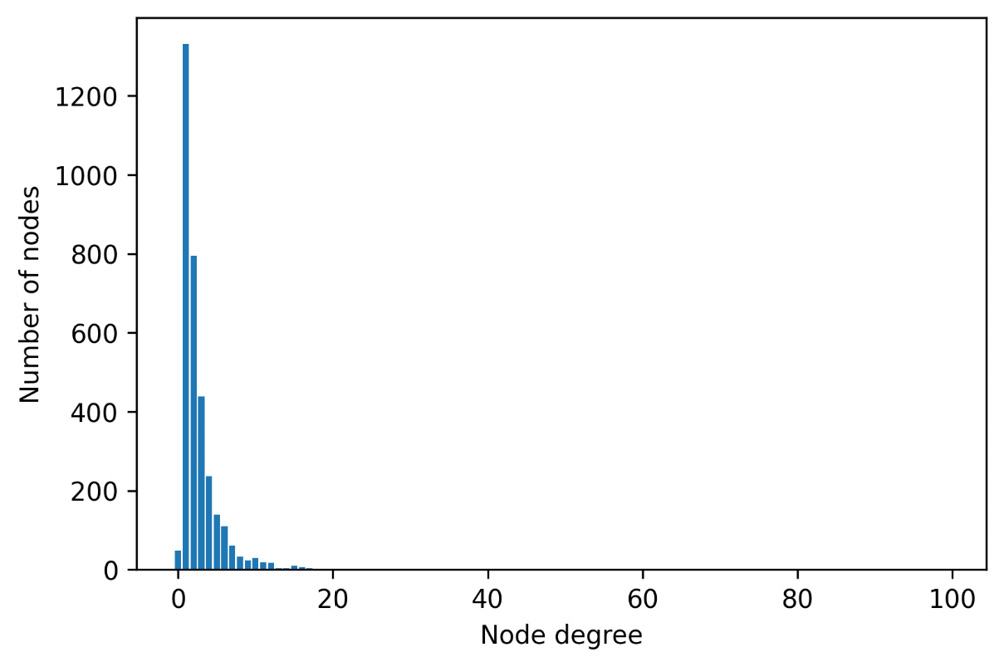
\includegraphics[width=\textwidth,height=0.72\textheight,keepaspectratio]{images/B19153_07_005.jpg}
\vspace{0.2em}

\small Figure 7.5 (교재): 데이터셋별 성능 차이 해석
\end{frame}

\begin{frame}{교재 그림: 결과 해석 포인트 (2)}
\centering
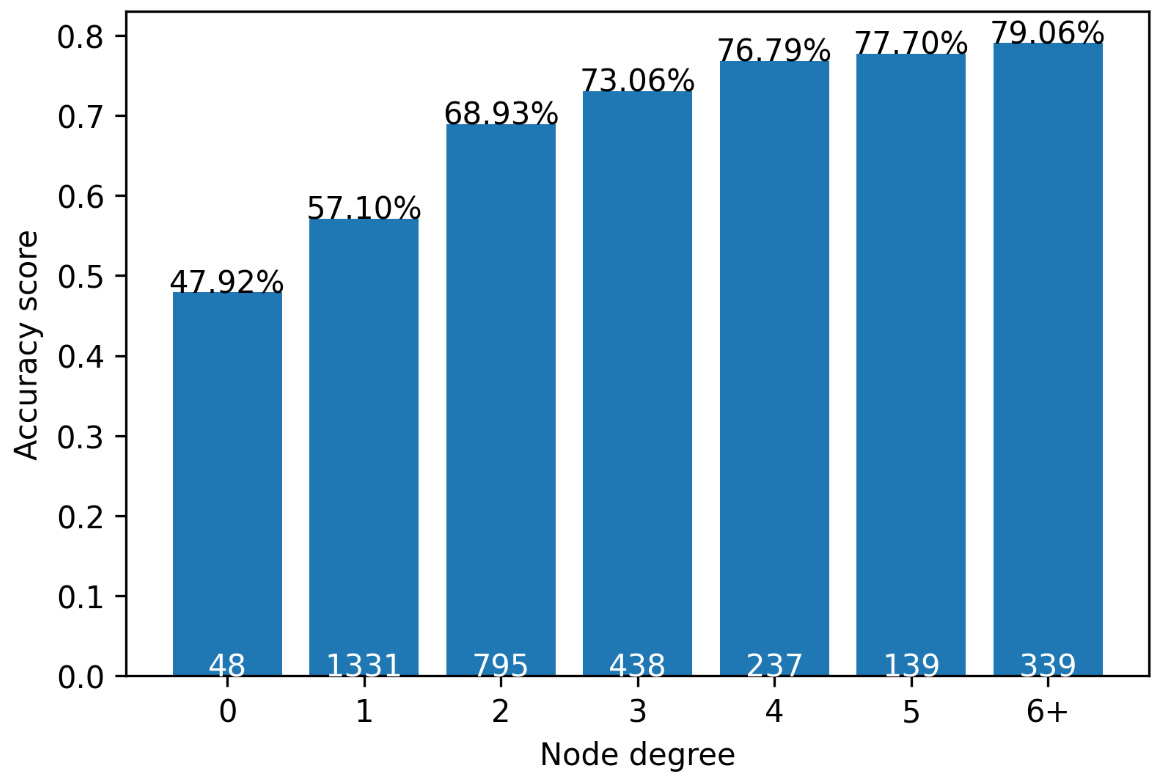
\includegraphics[width=\textwidth,height=0.72\textheight,keepaspectratio]{images/B19153_07_006.jpg}
\vspace{0.2em}

\small Figure 7.6 (교재): 모델 한계와 개선 관점
\end{frame}

\section{정리}

\begin{frame}{Chapter 7 핵심 정리}
\begin{itemize}
  \item GAT는 이웃 집계에 attention을 도입해 중요 이웃을 강조한다.
  \item 4노드 toy 예제로 $e_{ij}\rightarrow\alpha_{ij}$ 계산 직관을 확인했다.
  \item Cora/CiteSeer 실험으로 데이터셋별 성능 차이를 관찰했다.
  \item degree별 분석은 모델의 강점과 취약 구간을 해석하는 데 유용하다.
\end{itemize}
\end{frame}

\begin{frame}{발표 토론 질문}
\begin{itemize}
  \item GAT의 attention 계수는 언제 신뢰 가능한 해석 신호가 될까?
  \item heads 수, dropout, hidden dim은 성능/안정성에 어떻게 작용할까?
  \item heterophily 그래프에서도 같은 설정이 유효할까?
\end{itemize}
\end{frame}

\begin{frame}{바로 이어서 해볼 추가 실험}
\begin{enumerate}
  \item \texttt{heads=4, 8, 16} 비교
  \item \texttt{dropout=0.3, 0.6, 0.8} 비교
  \item 같은 split에서 \texttt{GATv2Conv}와 \texttt{GCNConv} 비교
  \item 오분류 노드의 degree와 이웃 라벨 분포 분석
\end{enumerate}
\end{frame}
